\documentclass[a4paper,11pt]{article} 
\usepackage{latexsym} 
\usepackage[MeX]{polski} 
\usepackage{indentfirst}
\usepackage{graphicx}
\usepackage[utf8]{inputenc}

\usepackage{fancyhdr}
\pagestyle{fancy}
\usepackage{lastpage}
\fancyfoot[C]{Page \thepage \hspace{1pt} of \pageref{LastPage}}

\graphicspath{ {images/} }
\author{Bartosz Michałowski} 
\title{
	\Huge Specyfikacja implementacyjna \\
	automat komórkowy\\
	\textbf{"WireWorld"}
} 
\frenchspacing     
\begin{document}
  %Strona tytułowa 
	\maketitle 
	\newpage
	\tableofcontents 
	\newpage
	\section {Informacje ogólne}
		\subsection{Nazwa programu}
			Nazwa programu:~\texttt{WireWorld}
		\subsection{Język}
		Program zostanie napisany w języku \textbf{Java}. W~programie nie przewiduje się zastosowania konstrukcji dostępnych w~\textbf{Javie wersji~8} i~wyższej. 
		\subsection{Uruchomienie programu}
				Program przeznaczony jest do uruchamiania za pomocą pliku \texttt{WireWorld.jar}.
		\newpage
    \section{Diagram pakietów}
    \begin{center}
 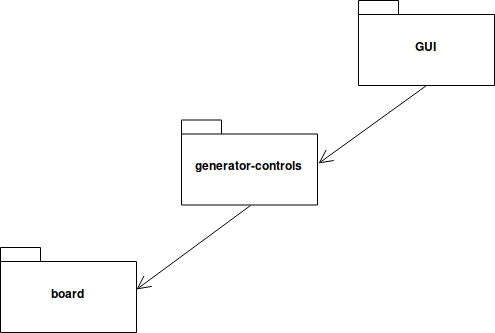
\includegraphics[scale=0.6]{images/diagram_pakiety.png}
 % diagram_pakiety.png: 495x333 px, 72dpi, 17.46x11.75 cm, bb=0 0 495 333
\end{center}

    \section{Opis pakietów}
        \subsection{Pakiet \texttt{GUI} }
            \subsubsection{Opis pakietu}
            Pakiet \texttt{GUI} zawiera klasy odpowiadające w~całości za~interfejs graficzny aplikacji. Klasą nadrzędną jest klasa GUI. Skorzystano z~biblioteki JavaFX.
            \subsubsection{Diagram klas}
            \begin{center}
 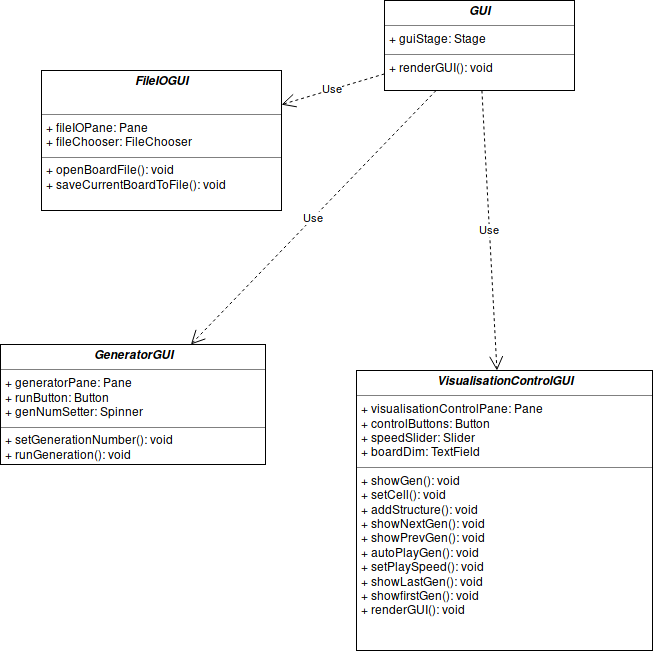
\includegraphics[scale=0.5]{images/pakiet_gui.png}
 % pakiet_gui.png: 653x651 px, 72dpi, 23.04x22.97 cm, bb=0 0 653 651
\end{center}

            \subsubsection{Opis klas}
                \begin{itemize}
                 \item Klasa \texttt{GUI} Jest to klasa opakowująca interfejs graficzny aplikacji w~celu zapewnienia przejrzystości i~ułatwienia tworzenia obsługi dla oddzielnych elementów programu.
                 \item Klasa \texttt{FileIOGUI} Udostępnia użytkownikowi elementy sterujące pozwalające wczytać nową bądź zapisać obecną generację z/do pliku w formacie obsługiwanym przez aplikację.
                 \item Klasa \texttt{GeneratorGUI} Udostępnia użytkownikowi dostęp do sterowania generatorem i modyfikację jego parametrów.
                 \item Klasa \texttt{VisualisationGUI} Klasa generująca interfejs sterujący wizualizacją generacji, przechodzeniem między kolejnymi stanami, określanie prędkości przechodzenia itp.
                \end{itemize}

        \subsection{Pakiet generation-controls}
            \subsubsection{\texttt{generation-controls}}
            Pakiet \texttt{generation-controls} odpowiada za~tworzenie kolejnych generacji planszy, możliwość eksportu ich do~pliku, udostępnienie interfejsu dla bibliotek graficznych oraz za~zapewnienie interfejsu umożliwiającego obsługę.
            \subsubsection{Diagram klas}
            \begin{center}
 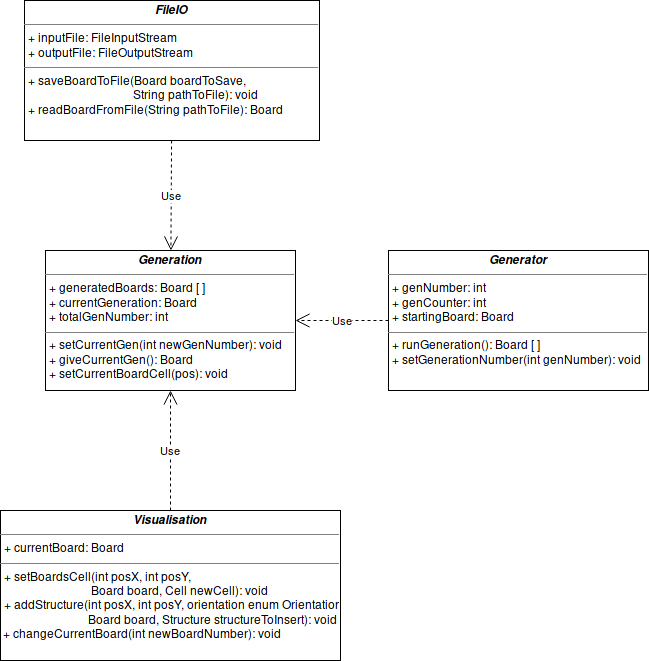
\includegraphics[scale=0.6]{images/pakiet_generation_controls.png}
 % pakiet_generation_controls.png: 649x661 px, 72dpi, 22.90x23.32 cm, bb=0 0 649 661
\end{center}

            \subsubsection{Opis klas}
            \begin{itemize}
             \item Klasa \texttt{Generator} Moduł zawierający algorytm generacji kolejnych stanów automatu, modyfikujący obiekt klasy \texttt{Board} opisanej w dalszej części specyfikacji.
             \item Klasa \texttt{FileIO} Klasa umożliwiająca zapis i odczyt plików z generacjami zawierająca odpowiedni do tych celów interfejs dostępny dla innych klas.
             \item Klasa \texttt{Visualisation} Przetwarza obiekt klasy \texttt{Board} na obiekt możliwy do reprezentacji graficznej dla obiektu klasy \texttt{VisualisationGUI}
             \item Klasa \texttt{Generation} Przechowuje generacje wynikowe pochodzące od klasy \texttt{Generation}.
            \end{itemize}

        \subsection{Pakiet\texttt{board}}
            \subsubsection{Opis pakietu}
            Pakiet \texttt{board} zapewnia struktury niezbędne do przechowywania danych na temat generacji, jak i ich modyfikację oraz odczyt.
            \subsubsection{Diagram klas}
            \begin{center}
 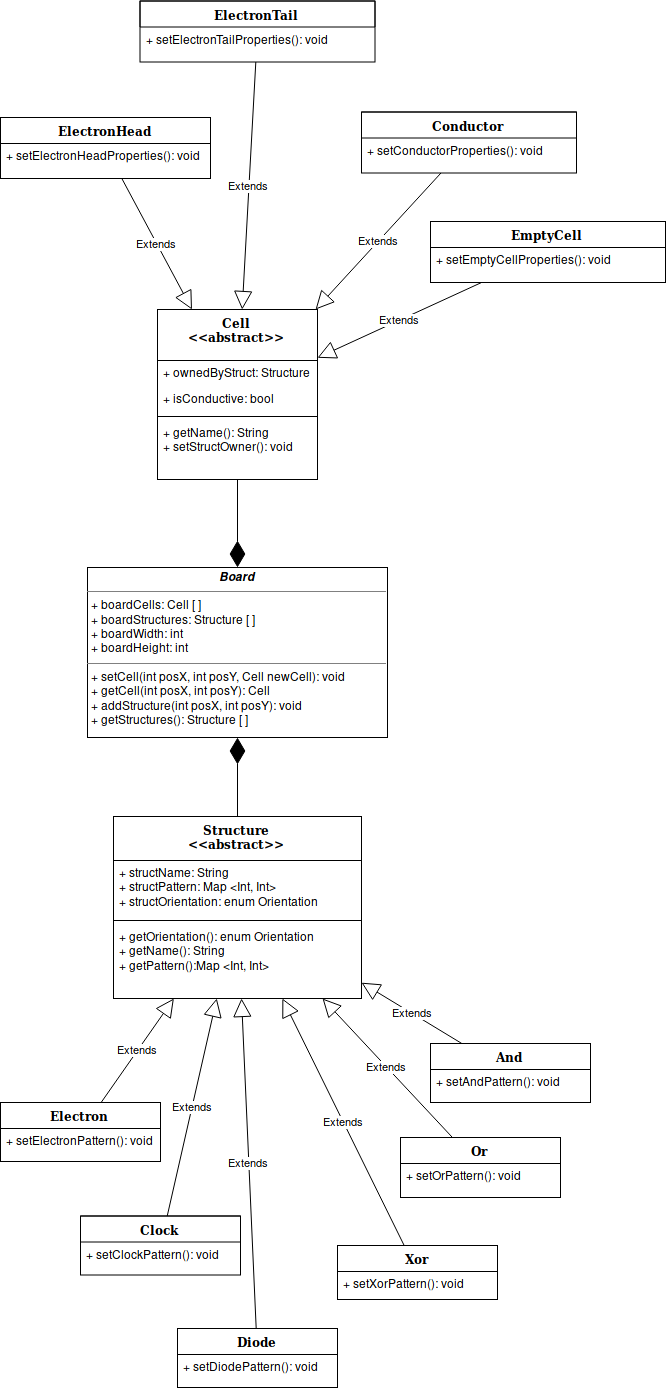
\includegraphics[scale=0.35]{images/pakiet_board.png}
 % pakiet_board.png: 666x1388 px, 72dpi, 23.50x48.97 cm, bb=0 0 666 1388
\end{center}

            \subsubsection{Opis klas}
            \begin{itemize}
             \item Klasa \texttt{Board} Klasa przechowująca wektor odpowiednich komórek oraz struktur generacji i udostępniająca interfejs pozwalający na ich odczytywanie i modyfikację.
             \item Klasa \texttt{Cell} Klasa abstrakcyjna reprezentująca pojedynczą komórkę i opakowująca ich różne rodzaje.
             \begin{enumerate}
              \item Klasa \texttt{ElectronHead} Klasa rozszerzająca klasę \texttt{Cell} o komórkę przedstawiającą głowę elektronu.
              \item Klasa \texttt{ElectronTail} Klasa rozszerzająca klasę \texttt{Cell} o komórkę przedstawiającą ogon elektronu.
              \item Klasa \texttt{Conductor}  Klasa rozszerzająca klasę \texttt{Cell} o komórkę symbolizującą przewodnik.
              \item Klasa \texttt{EmptyCell}  Klasa rozszerzająca klasę \texttt{Cell} o pustą komórkę niebędącą przewodnikiem.
             \end{enumerate}
             \item Klasa \texttt{Structure} Klasa abstrakcyjna reprezentująca struktury składająca się z obiektów klas rozszerzających klasę \texttt{Cell} wraz z ich odpowiednimi pozycjami.
             \begin{enumerate}
              \item Klasa \texttt{Electron}  Klasa rozszerzająca klasę \texttt{Structure} o elektron składający się z głowy i ogona.
              \item Klasa \texttt{Diode} Klasa rozszerzająca klasę \texttt{Structure} o strukturę przepuszczającą elektrony tylko w jednym kierunku.
              \item Klasa \texttt{Clock} Klasa rozszerzająca klasę \texttt{Structure} o strukturę generującą periodycznie elektrony.
              \item Klasa \texttt{OR} Klasa rozszerzająca klasę \texttt{Structure} o bramke logiczną OR.
              \item Klasa \texttt{XOR} Klasa rozszerzająca klasę \texttt{Structure} o bramke logiczną XOR.
              \item Klasa \texttt{AND} Klasa rozszerzająca klasę \texttt{Structure} o bramke logiczną AND.
             \end{enumerate}
            \end{itemize}

    \section{Przechowywanie danych w programie i metoda generacji}
        \subsection{Przechowywanie danych w programie}
        Dane na temat generacji przechowywane~są w~obiekcie klasy \texttt{Generation} w~postaci listy kolejnych stanów klasy \texttt{Board}, które z~kolei zawierają informację na~temat stanu komórek oraz zawartych w~danej tablicy struktur. Przechowywanie informacji na~temat struktur pozwala zapisać ich~pozycje do~pliku wyjściowego. W~razie modyfikacji pola należącego do~struktury, jest~ona usuwana z~generacji i~dalej reprezentowana jedynie jako pola, które nie~uległy modyfikacji.
        \subsection{Metoda generacji}
        Algorytm przechodzi po~kolejnych polach obiektu klasy \texttt{Board} sprawdzając~czy nie~jest on~polem pustym. Jeśli warunek~ten jest spełniony pole modyfikowane jest na~podstawie stanu komórek sąsiednich. Po~przejściu całego obiektu jest on~zapisywany jako kolejny stan w~obiekcie klasy \texttt{Generation}.
	\section{Wymagania dotyczące użytkowania programu}
		Program jest przenośny, przez co~rozumie się, że może zostać uruchomiony na każdym komputerze, który posiada zainstalowane \texttt{Java Runtime Environment (JRE)}, co w~wolnym tłumaczeniu można określić jako \textsl{środowisko uruchamiania Java}. Jeżeli wyżej wymienione środowisko jest zainstalowane na danym komputerze to spełnia on wymagania systemowe odnośnie funkcjonowania programu. Program przeznaczony jest do uruchamiania za pomocą pliku \texttt{WireWorld.jar}. 
	\section{Testowanie}
		Testowanie wodzące w projekcie to testowanie jednostkowe i~użytkownika końcowego. Celem fazy testowania będzie sprawdzenie czy dana, tworzona przez nas funkcjonalność działa zgodnie z~jej przeznaczeniem. Procesy testowania  przeprowadzimy samodzielnie, głównie z~użyciem narzędzi \textsl{JUnit}, \textsl{Mockito} i~\textsl{AssertJ}.
		\subsection{Konwencja}
		Procesy testowania jednostkowego będą przebiegały z~podstawowymi założeniami dobrych praktyk, będziemy tworzyć testy, które są niezależne od siebie, począwszy od najprostszych do najtrudniejszych funkcjonalności. Nazwy metod testujących będą starały się zobrazować oczekiwany efekt. Interfejs graficzny zostanie przetestowany ręcznie, sprawdzając czy interakcja z~odpowiednimi jego elemantami zgadza się z~przewidywanym rezultatem.
		\subsection{Narzędzia}
		Narzędzia użyte w~procesie testowania to:
		\begin{enumerate}
			\item Biblioteka \textsl{JUnit}
			\item Biblioteka \textsl{AssertJ}
			\item Biblioteka \textsl{Mockito}
		\end{enumerate}
	\section{Wersjonowanie}
		Wersjonowanie projektu jest oparte o~system kontroli wersji \textsl{Git}. Wersje programu są~przechowywane w repozytorium \texttt{2018\_JIMP2\_repozytorium\_gr1} stworzonym na~potrzeby projektu. Kolejne wersje umieszczono w gałęzi \texttt{master} wyżej wymienionego repozytorium.
	\section{Narzędzia}	
	Narzędzie użyte w~procesie tworzenia programu to:
	\begin{enumerate}
		\item Zintegrowane środowisko deweloperskie \textsl{IntelliJ IDEA}
		\item System kontroli wersji \textsl{Git}
		\item Biblioteka \textsl{JUnit}
		\item Biblioteka \textsl{AssertJ}
		\item Biblioteka \textsl{Mockito}
		\item Biblioteka \textsl{Maven}
		\item Biblioteka \textsl{Apache Ant}
		\item Biblioteka \textsl{JavaFX}
	\end{enumerate}
	
\end{document}
